\documentclass[paper=a4, fontsize=11pt,twoside]{article}

% -------------------------------------------------------------------- 
% General Page Layout
% --------------------------------------------------------------------
\usepackage[a4paper]{geometry} 
\usepackage[parfill]{parskip}
\setlength{\oddsidemargin}{5mm}  % Remove 'twosided' indentation
\setlength{\evensidemargin}{5mm}

% --------------------------------------------------------------------
% Encoding and Language Settings
% --------------------------------------------------------------------
\usepackage[T1]{fontenc} 
\usepackage[utf8]{inputenc}   
% encoding may need to be changed depending on the system
\usepackage[swedish]{babel} 
\usepackage{lipsum} % Lorem Ipsum

% --------------------------------------------------------------------
%  Utilities (colors, links, pictures, ect...)
% --------------------------------------------------------------------
\usepackage{xcolor}
\usepackage{hyperref}
\usepackage{graphicx}
\usepackage{amssymb}
\usepackage{epstopdf}
\usepackage[round]{natbib}
\usepackage{float}
\DeclareGraphicsRule{.tif}{png}{.png}{`convert #1 `dirname #1`/`basename #1 .tif`.png}

% -----------------------------------------------------------------------------%
% Title Page / Document Class Definitions (Please Don't Play With This)
% -----------------------------------------------------------------------------%
	
% Table of contents depth = section & subsection
\setcounter{tocdepth}{2}
																								
% Horizontal rule
\newcommand{\HRule}[1]{\rule{\linewidth}{#1}}   															
																											
% Document Number
\newcommand{\documentNumber}[1]{\centering PUSP1742#1 \\[1.0cm]}	 										
																											
% Document Version
\newcommand{\documentVersion}[1]{\centering \small{v.#1} \\[1.0cm]}

% Group Responsible
\newcommand{\documentResponsible}[1]{\centering  Ansvarig Grupp: #1}

% Document Creator Group
\newcommand{\documentCreator}[1]{\centering Uppgjord Av: #1}	 									
																										
% Title
\makeatletter \def\printtitle{ {\centering \@title\par}} \makeatother
																											
% Author .. not really used, but it can stay in case
\makeatletter \def\printauthor{ {\centering \large \@author}} \makeatother
																											
\newcommand{\grouptitlepage}[4]{ 
	\title{
		\documentNumber{#1}																						
		\documentVersion{#2}																				
		\HRule{0.5pt} \\ % Upper rule 
		\LARGE \textbf{\uppercase{#3}} \\
		\large \textbf{\uppercase{ETSF20 Grupp 2}} 
		\HRule{2pt} \\ [1.5cm]    
		\normalsize            
		\documentResponsible{#4} \\ 
		\documentCreator{#4}  
	}																							
	\maketitle																							
	\thispagestyle{empty} 																					
	\newpage 
}
% \grouptitlepage{doc number}{Version Number}{doc title}{group responsible for
% doc}
% --------------------------------------------------------------------------------%
% Title Page / Document Class Definitions (Please Don't Play With This)
% --------------------------------------------------------------------------------%


% \date{}                                            
% Activate to display a given date or keep commented for current date


% -------------------------------------------------------
% DOCUMENT START (YOU CAN IGNORE EVERYTHING ABOVE HERE)
% -------------------------------------------------------
\begin{document}

% ---------------------------------------------------------------------------------------------------------------------------------------
% Title Page START: \grouptitlepage{doc number}{Version Number}{doc title}{group responsible for doc}		
% ---------------------------------------------------------------------------------------------------------------------------------------
\grouptitlepage
%Document Code Number (same as time reports)
{13}
%Document Version Number										
{0.2}
%Document Title		Dokumentmall							
{SVVS - Testspecifikation}
%Group Responsible For Document									
{(TG) Test Grupp} %ö
% -------------------------------------------------------------------------------------------------------------
% Title Page END				
% -------------------------------------------------------------------------------------------------------------
\tableofcontents
\section{Introduktion}

 Detta dokument beskriver hur ett system baserat på “BaseBlockSystem”
 ska verifieras.
 

\section{Referensdokument}

\begin{enumerate}
\item Projekthandledning
\item SRS v 0.1
\end{enumerate}

\section{Överblick}   %ö
Under projektets gång kommer tre formella granskningar genomföras.
\begin{enumerate}
\item Software Specication Review (SSR)
	\begin{enumerate}
	\item SDP
	\item SRS
	\item SVVS
	\end{enumerate}
\item Preliminary Design Review(PDR)
	\begin{enumerate}
	\item SVVI
	\item SSD
	\end{enumerate}
\item Product Review (PR)
	\begin{enumerate}
	\item SVVR
	\item SSD
	\item PFR
	\end{enumerate}
\end{enumerate}
Dessa formella granskningar genomförs som de har beskrivits i Ref.1. Varje
formell granskning kommer föregås av en informell granskning utan närvaro av
kundens representanter, som beskrivs i Ref 1. De informella granskningarna “är
planerade så att uppdaterat material kan levereras” till formell granskning.
Utöver de informella granskningarna som anges ovan så ska även SDDD ses över av
utvecklingsgruppen.
\section{Test}

\subsection{Testmiljöer}

Under projektet kommer olika testmiljöer att användas. Dessa kommer att innefatta

\begin{itemize}
\item \textbf{Webbläsare (Internet Explorer 10,Google Chrome)}
\item \textbf{Junit}
\item \textbf{Operativsystem (Microsoft Windows 10, IOS)}
\item \textbf{Server System (Apache Tomcat)}
\end{itemize}

\subsection{Testfall}

Testerna kommer att genomföras i följande faser:

{\bf Enhetstest:} Dessa testerna utförs direkt av UG på utvecklad programvara
innan den har implementerats i systemet. Detta görs informellt och kräver därför ingen dokumentation.

{\bf Funktionstest:} Här testas enstaka funktioner så långt de är utvecklade
innan de är implementerade i resten av systemet.

{\bf Systemtest:} Här genomförs allmänna tester på hela systemet. 

{\bf Regressionstest:} Alla angivna testfall genomförs på nytt för varje
uppdatering som görs på systemet.

{\bf Acceptanstest:} Dessa tester genomför av institutionen under den sista
granskning(PR) Här kommer alla angivna testfall användas tillsammans med egna testfall som beslutas av institutionen.

 
\section{Kontrollkrav för granskning}

Under granskning ska alla krav kontrolleras av granskaren.

\section{Appendix}

\begin{itemize}
\item[\bf A.] Specifikation av funktionstest
\item[\bf B.] Tabeller
\end{itemize}

\section*{A Specifikation av funktionstest}

\subsection{Administratör}
\begin{itemize}
\item[FT1] Kan skapa projektgrupper [SRS 9.1.1] 
\item[FT2] Kan ta bort projektgrupper [SRS 9.1.2] 
\item[FT3] Tilldelar rollen PG i en projektgrupp [SRS 9.1.3, 9.1.4]
\item[FT4] Lägger till och tar bort användare från systemet [SRS 9.1.5, 9.1.6,
9.1.8]
\item[FT5] Kan ej ta bort sig själv [SRS 9.1.7]
\end{itemize}

\subsection{Projektledare}  
\begin{itemize}
\item[FT6] Kan endast tilldela följande roller till projektmedlemmar i projektgruppen ref Appendix B 9.3 [SRS 9.1, 9.2.2]
\item[FT7] Kan ändra roller i projektgruppen ref Appendix B 9.3 [SRS 9.2.3, 9.2.4]
\item[FT8] Kommer åt sin meny ref Appendix B 9.4 [SRS 9.2.10] 
\item[FT9] Försöker tilldela fler roller till samma projektmedlem [SRS 9.3.6] 
\item[FT10] Kan attestera rapport [SRS 9.2.5, 9.2.6, 9.2.7, 9.2.8] 
\item[FT11] Kan annulera en attesterad rapport [SRS 9.2.9] 
\item[FT12] Kan se allas statistik i sin projektgrupp ref Appendix B 9.5 [SRS 9.2.11, 9.2.12, 9.2.13, 9.2.14]
\end{itemize}


\subsection{Användare} 
\begin{itemize}
\item[FT13] Kan lämna in tidsrapport [SRS 9.3.1, 9.3.2] 
\item[FT14] Kan uppdatera sin tidsrapport innan attestering [SRS 9.3.3,
9.3.4, 9.3.7]
\item[FT15] Kan se sin statistik [SRS 9.3.5, 9.3.8] 
\item[FT16] Ändra lösenord [SRS 9.3.9, 9.3.10] 
\end{itemize}

\section{Kvalitetskrav} 
\begin{itemize}
\item[FT17] Systemet uppfyller den förväntade svarstiden vid LTH Campus Helsingborg
[SRS 7.1.1]
\end{itemize}

\section{Projektkrav} 
\begin{itemize}
\item[FT18] Systemet uppfyller användarbarhetskraven [SRS 9.0.1] 
\item[FT19] Systemet är en vidareutveckling av grundsystemet [SRS 6.1.2]
\item[FT20] Ny loggfil skapas när ny projektgrupp skapas [SRS 9.0.2]
\item[FT21] Loggfilen för projektgruppen uppdateras för varje ändring i
projektgruppen [SRS 9.0.3]
\item[FT22] Loggfilen raderas när en projektgrupp raderas från systemet [SRS
9.0.4] 
\item[FT23] Ett inlägg i loggfilen innehåller tidsstämpel samt användare [SRS
9.0.5]
\end{itemize}

\section{Designkrav} 

\subsection{}
Designkrav uppfylls ref 2 figur 2 [SRS 8.1.1]
\subsection{}
Designkrav uppfylls ref 2 figur 3 [SRS 8.1.2]
\section*{B Tabeller}

\subsection{ }
\begin{enumerate}
\item[]
	\begin{enumerate}
	\item Projektgrupp
	\item Systemgrupp
	\item Utvecklingsgrupp
	\item Testgrupp
	\end{enumerate}
\end{enumerate}

\subsection{ }
\begin{enumerate}
\item[]
	\begin{enumerate}
	\item Organize Group
	\item Sign report
	\item Unsign reports
	\item View all reports
	\end{enumerate}
\end{enumerate}

\subsection{ }

\begin{enumerate}
\item[]
	\begin{enumerate}
	\item Användare
	\item Roll
	\item Aktivitet
	\item Vecka
	\item Fas
	\item Dokument
	\end{enumerate}
\end{enumerate}


\section{Test/krav matris}
\begin{figure}[H]
\centering
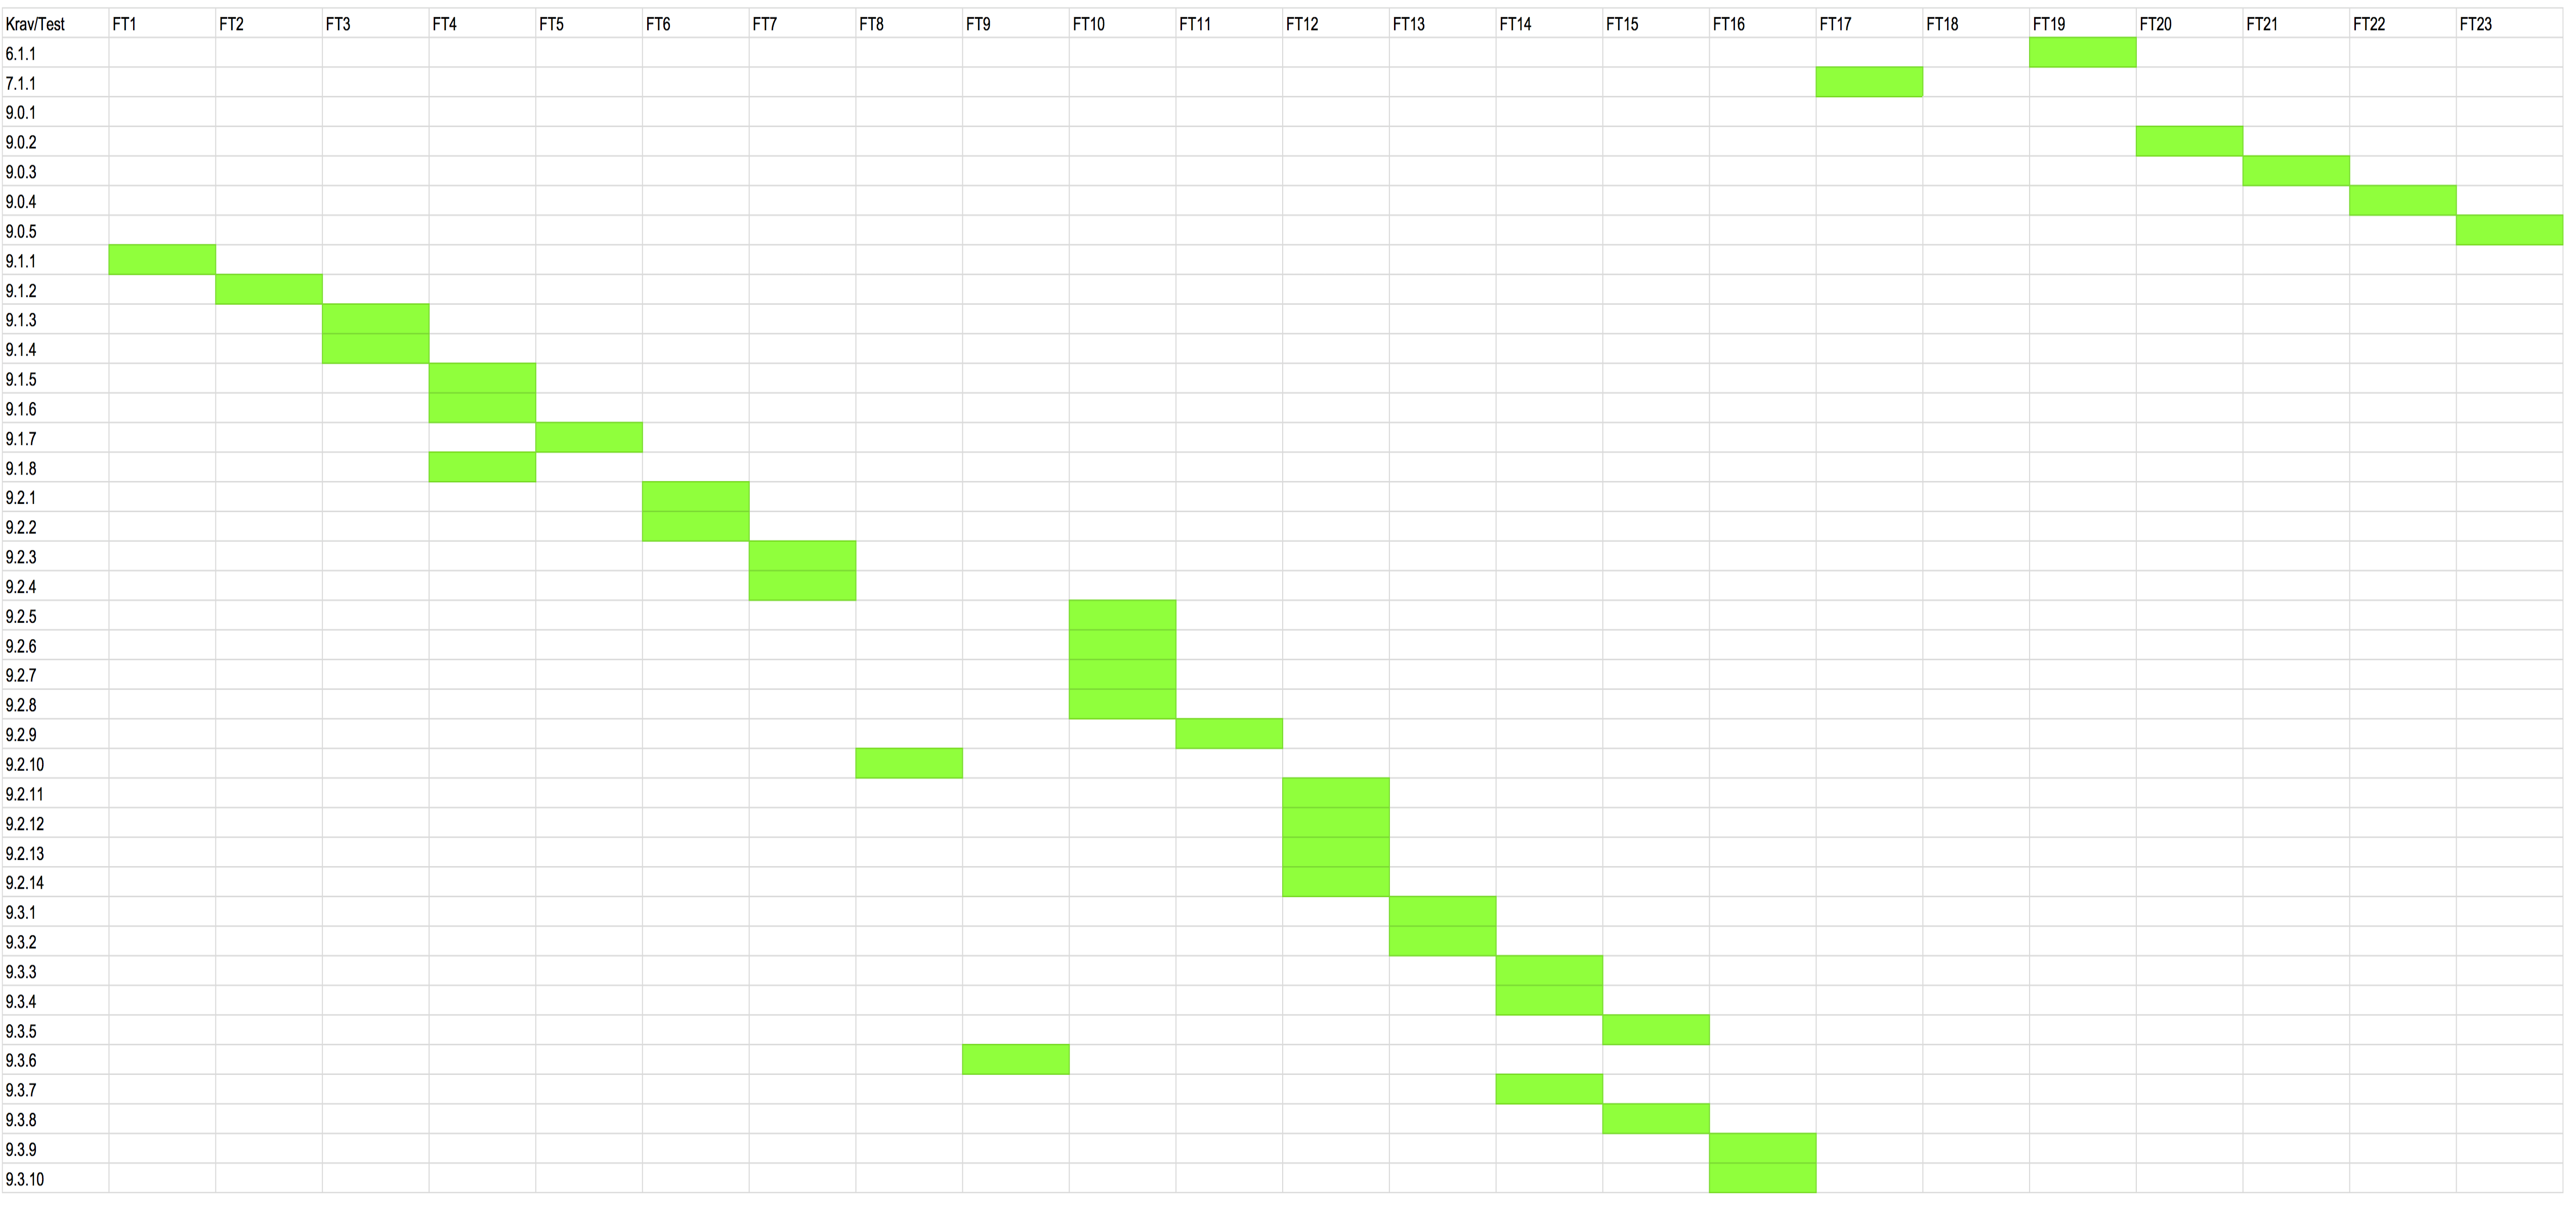
\includegraphics[width = 16cm]{SVVS_Matris.png} %height=6cm,
\caption{Test/krav matris}
\end{figure}


\end{document}
